\documentclass[12pt, a4paper]{article}
\usepackage{amsmath}
\usepackage{amssymb}
\usepackage[utf8]{inputenc}    % Soporte para caracteres especiales
\usepackage{amsfonts}
\usepackage[right=3cm, left=2.5cm, top=3cm, bottom=3.5cm]{geometry}
\usepackage{graphicx}
\usepackage[spanish,english]{babel}
\usepackage{csquotes}
\usepackage{setspace}
\usepackage{float}
\usepackage{apacite}
\bibliographystyle{apacite}

%\usepackage{hyperref} % Enlaces y referencias
%\usepackage[style=apa]{biblatex}
%\usepackage{csquotes}          % Manejo de citas (opcional, útil para biblatex)
%\addbibresource{references.bib}
%\usepackage[spanish]{babel}
\title{Cuales son los beneficios y los riesgos
de la resonancia magnética en el cuerpo}
\author{Torres Tarrillo Rober}

\begin{document}
\begin{titlepage}
\begin{center}

% --- Logos y encabezado superior ---
\begin{minipage}{0.2\textwidth}
    \begin{flushleft}
        \includegraphics[width=\linewidth]{img/logounp.png}
    \end{flushleft}
\end{minipage}
\begin{minipage}{0.6\textwidth}
    \begin{center}
        \vspace{2cm}
        \textbf{\large UNIVERSIDAD NACIONAL DE PIURA}\\[0.3cm]
        \vspace{0.3cm}
        \textbf{\large FACULTAD DE CIENCIAS}\\[0.3cm]
        \vspace{1cm}
        \textbf{ ESCUELA PROFESIONAL DE FÍSICA}
    \end{center}
\end{minipage}
\begin{minipage}{0.17\textwidth}
    \begin{flushright}
        \includegraphics[width=\linewidth]{img/physics.png}
    \end{flushright}
\end{minipage}

\vspace{2cm}

% --- Título ---
{\Large \textbf{
    Laboratorio virtual de espectrofotometría UV-VIS    
}}\\[1.5cm]

% --- Docente ---
\textbf{Docente:}\\ Dr. Quispe Moreno, Gustavo\\[1cm]

% --- Alumnos ---
\textbf{Alumnos:}\\
Torres Tarrillo, Rober E.\\
Carcamo Calderon, Andri, J.\\

% --- Fecha y lugar ---
\vfill
Piura, Diciembre 2025

\end{center}
\end{titlepage}
    

\selectlanguage{spanish}
\begin{abstract}
La resonancia magnética (RMN) es una de las técnicas de diagnóstico más avanzadas de la medicina moderna. Este trabajo analiza los principios físicos, las aplicaciones médicas, los beneficios y los posibles riesgos asociados con la RMN. Se destaca que la resonancia magnética permite obtener imágenes de alta resolución de los tejidos internos sin utilizar radiación ionizante, lo que la hace especialmente útil para el estudio del cerebro, la médula espinal, las articulaciones y los tejidos blandos. Entre sus principales ventajas se encuentran la detección temprana de enfermedades y la posibilidad de realizar estudios funcionales del cuerpo humano. Sin embargo, la RMN presenta ciertos riesgos y limitaciones, como la interferencia magnética con implantes metálicos, reacciones alérgicas a los agentes de contraste y el elevado costo de los equipos. El análisis concluye que, a pesar de sus desafíos, la resonancia magnética sigue siendo una herramienta segura y de gran valor en el diagnóstico médico cuando se aplica bajo protocolos adecuados de seguridad.

\textbf{Palabras clave:} resonancia magnética, diagnóstico médico, beneficios, riesgos, radiología
\end{abstract}

\newpage
\tableofcontents
\newpage
\section{Introducción}

La resonancia magnética (RMN) constituye una de las herramientas más importantes en el diagnóstico médico contemporáneo. Desde su desarrollo en la década de 1970, esta técnica ha revolucionado la forma en que los profesionales de la salud observan el interior del cuerpo humano, permitiendo obtener imágenes detalladas de los tejidos blandos sin la necesidad de procedimientos invasivos ni el uso de radiación ionizante. Su aplicación se ha extendido ampliamente en áreas como la neurología, la cardiología, la oncología y la ortopedia, convirtiéndose en un pilar esencial para el diagnóstico temprano y el seguimiento de diversas patologías.

En la actualidad, la resonancia magnética adquiere una relevancia cada vez mayor debido a la necesidad de métodos diagnósticos más seguros, precisos y no invasivos. Comprender los beneficios que ofrece y los riesgos que puede implicar resulta fundamental tanto para los profesionales de la salud como para los pacientes, ya que permite un uso responsable y ético de esta tecnología. Además, su importancia trasciende el ámbito clínico, al involucrar también aspectos físicos, tecnológicos y económicos que influyen en su implementación en los sistemas de salud.

El objetivo principal de este trabajo es analizar los beneficios y los riesgos de la resonancia magnética en el cuerpo humano, considerando sus fundamentos físicos, su impacto en el diagnóstico médico y las posibles limitaciones que presenta. Asimismo, se busca promover una reflexión sobre la necesidad de equilibrar la precisión diagnóstica con la seguridad del paciente.

El contenido de esta monografía se organiza en varias secciones. En primer lugar, se presenta el marco teórico, donde se explican los principios físicos y tecnológicos que sustentan la resonancia magnética. Posteriormente, se desarrollan los apartados dedicados a sus beneficios clínicos y a los riesgos potenciales asociados con su uso. Finalmente, se exponen las conclusiones generales y las recomendaciones que surgen del análisis realizado.

\section{Marco teórico}

\subsection{Definición y principios físicos de la resonancia magnética}

La resonancia magnética (RM) es una técnica espectroscópica basada en la interacción de los momentos magnéticos nucleares con un campo magnético externo intenso. En medicina, esta técnica se adapta para generar imágenes tridimensionales del cuerpo humano sin recurrir a radiación ionizante. Su principio fundamental es la \textbf{resonancia magnética nuclear (RMN)}, fenómeno físico que describe cómo los núcleos con momento magnético intrínseco absorben y reemiten energía en forma de ondas de radio cuando se encuentran en un campo magnético estático.

\subsubsection*{Fundamento físico}

El momento magnético nuclear \(\vec{\mu}\) está relacionado con el momento angular nuclear \(\vec{I}\) mediante:

\[
\vec{\mu} = \gamma \vec{I}
\]

donde \(\gamma\) es la \textit{razón giromagnética} característica de cada tipo de núcleo.  
En presencia de un campo magnético externo uniforme \(\vec{B}_0\), el momento magnético experimenta una interacción descrita por la energía potencial:

\[
E = - \vec{\mu} \cdot \vec{B}_0 = - \gamma \hbar m_I B_0
\]

donde \(m_I\) representa el número cuántico magnético.  
La separación energética entre los dos estados de espín (para núcleos con \(I = \tfrac{1}{2}\), como el protón) es:

\[
\Delta E = \gamma \hbar B_0
\]

Cuando el sistema se irradia con una onda de radiofrecuencia de frecuencia \(\nu\), se produce absorción resonante si:

\[
h\nu = \Delta E \Rightarrow \nu = \frac{\gamma B_0}{2\pi}
\]

Esta ecuación, conocida como \textbf{condición de resonancia de Larmor}, determina la frecuencia a la cual los núcleos entran en resonancia con el campo aplicado.  
El movimiento de precesión del vector magnetización alrededor de \(\vec{B}_0\) ocurre precisamente a esta frecuencia \(\omega_0 = \gamma B_0\).

\subsubsection*{Componentes básicos del equipo}

Un sistema de resonancia magnética está compuesto por los siguientes elementos principales:

\begin{itemize}
    \item \textbf{Imán principal:} genera el campo magnético estático \(\vec{B}_0\), típicamente entre 1.5 y 3~T en equipos clínicos.
    \item \textbf{Bobinas de gradiente:} producen campos magnéticos variables espacialmente, permitiendo codificar la posición de los núcleos en las tres direcciones del espacio.
    \item \textbf{Bobinas de radiofrecuencia (RF):} emiten los pulsos de excitación y reciben las señales emitidas por los núcleos.
    \item \textbf{Sistema computacional:} realiza la reconstrucción de imágenes mediante transformadas de Fourier de las señales recibidas, generando cortes anatómicos de alta resolución.
\end{itemize}

\begin{figure}[H]
    \centering
    \includegraphics[width=1\textwidth]{img/2.png}
    \caption{Equipo de resonancia magnética, partes y funcionamiento.}
\end{figure}


\subsubsection*{Diferencias con los rayos X y la tomografía}

A diferencia de los rayos X o la tomografía computarizada (TC), la resonancia magnética no utiliza radiación ionizante, sino ondas de radio de baja energía.  
Mientras que los rayos X se basan en la absorción diferencial de radiación por los tejidos, la RM depende de las propiedades magnéticas y de relajación de los núcleos, denominadas tiempos de relajación \(T_1\) (longitudinal) y \(T_2\) (transversal), que caracterizan la recuperación de la magnetización tras la excitación:

\[
M_z(t) = M_0 \left(1 - e^{-t/T_1}\right), \quad M_{xy}(t) = M_0 e^{-t/T_2}
\]

Estas constantes permiten obtener contrastes entre diferentes tipos de tejidos, lo que convierte a la RM en una herramienta altamente sensible para el diagnóstico médico.

\subsection{Historia y desarrollo tecnológico}

El fenómeno de resonancia magnética fue descubierto en 1946 de forma independiente por Felix Bloch y Edward Purcell, quienes demostraron que los núcleos atómicos absorbían energía en presencia de un campo magnético y una radiación de frecuencia adecuada. Este hallazgo, en el contexto de la espectroscopía nuclear, les valió el Premio Nobel de Física en 1952.

Durante la década de 1970, Raymond Damadian y Paul Lauterbur aplicaron el principio de resonancia magnética a la obtención de imágenes, utilizando gradientes de campo para localizar señales en el espacio. Posteriormente, Peter Mansfield desarrolló técnicas de adquisición rápida y reconstrucción por transformada de Fourier, lo que permitió la formación eficiente de imágenes tridimensionales. Por estos avances, Lauterbur y Mansfield recibieron el Premio Nobel de Fisiología o Medicina en 2003.

En la actualidad, las mejoras en la tecnología de imanes superconductores, la electrónica de radiofrecuencia y los algoritmos de reconstrucción han permitido el desarrollo de variantes avanzadas como:

\begin{itemize}
    \item \textbf{Resonancia magnética funcional (RMf):} mide cambios en la oxigenación sanguínea para mapear la actividad cerebral.
    \item \textbf{Espectroscopía por resonancia magnética (ERM):} permite analizar metabolitos en tejidos y órganos.
    \item \textbf{Resonancia magnética de difusión:} estudia la movilidad molecular del agua, útil en el diagnóstico de lesiones cerebrales.
\end{itemize}

Estas variantes extienden el alcance de la RM más allá de la imagen anatómica, hacia el estudio dinámico y funcional del cuerpo humano, conectando directamente con los fundamentos de la espectroscopía nuclear.


\section{Beneficios de la resonancia magnética}

La resonancia magnética (RM) representa uno de los mayores avances tecnológicos en el diagnóstico médico moderno. Su principio no invasivo y su capacidad para diferenciar tejidos blandos con una resolución espacial excepcional la convierten en una herramienta de gran valor tanto en la práctica clínica como en la investigación científica.  
En términos físicos, la RM aprovecha las diferencias en los tiempos de relajación \(T_1\) y \(T_2\) de los protones para generar contrastes entre tejidos, lo cual proporciona información morfológica y funcional sin necesidad de procedimientos invasivos ni radiación ionizante.

\subsection{Diagnóstico preciso y no invasivo}

Uno de los principales beneficios de la resonancia magnética es su capacidad para obtener imágenes con alta resolución espacial y excelente contraste de tejidos blandos. Esto se debe a la sensibilidad del método frente a los parámetros de relajación nuclear, definidos por las ecuaciones:

\[
M_z(t) = M_0\left(1 - e^{-t/T_1}\right), \qquad M_{xy}(t) = M_0 e^{-t/T_2}
\]

Estas expresiones describen cómo el vector de magnetización longitudinal (\(M_z\)) y transversal (\(M_{xy}\)) se recuperan o decaen tras la excitación de los espines nucleares.  
Las diferencias en \(T_1\) y \(T_2\) entre tejidos permiten obtener contrastes precisos entre estructuras como cerebro, médula espinal, músculos, hígado o articulaciones.

A diferencia de los métodos basados en radiación ionizante —como los rayos X o la tomografía computarizada— la RM utiliza ondas de radio, cuya energía es del orden de los megahercios, lo que evita efectos de ionización y daño celular. Por ello, puede repetirse de forma segura en estudios de seguimiento o en pacientes pediátricos.

\begin{figure}[H]
    \centering
    \includegraphics[width=0.6\textwidth]{img/cerebro_rm.png}
    \caption{Imagen por resonancia magnética del cerebro humano, donde se observa la diferenciación entre sustancia gris y blanca.}
    \label{fig:cerebro_rm}
\end{figure}

\subsection{Aplicaciones médicas}

La versatilidad de la resonancia magnética ha permitido su aplicación en múltiples campos de la medicina moderna:

\begin{itemize}
    \item \textbf{Neurología:} la RM es fundamental en la detección de tumores cerebrales, esclerosis múltiple y accidentes cerebrovasculares. Su alta resolución permite observar la morfología cortical y el flujo sanguíneo cerebral.
    \item \textbf{Cardiología:} mediante secuencias de sincronización con el ciclo cardíaco, es posible estudiar la función ventricular, el flujo en arterias coronarias y la perfusión miocárdica.
    \item \textbf{Oncología:} la RM es una herramienta clave para la localización y caracterización de tumores en tejidos blandos, especialmente en cerebro, mama y próstata, permitiendo evaluar su extensión sin biopsias invasivas.
    \item \textbf{Ortopedia:} las imágenes por RM muestran con precisión lesiones musculares, ligamentarias y cartilaginosas, siendo esenciales en el diagnóstico deportivo y traumatológico.
\end{itemize}

\begin{figure}[H]
    \centering
    \includegraphics[width=0.6\textwidth]{img/rodilla_rm.png}
    \caption{Imagen de resonancia magnética de rodilla. Se distingue claramente el cartílago articular, los ligamentos y los meniscos.}
    \label{fig:rodilla_rm}
\end{figure}

\subsection{Avances recientes}

En las últimas décadas, la resonancia magnética ha evolucionado hacia técnicas especializadas que amplían sus capacidades diagnósticas y experimentales:

\begin{itemize}
    \item \textbf{Resonancia magnética funcional (RMf):} permite mapear la actividad cerebral midiendo variaciones en la oxigenación sanguínea (\textit{efecto BOLD, Blood Oxygen Level Dependent}). Este fenómeno se basa en la diferente susceptibilidad magnética de la oxihemoglobina y la desoxihemoglobina, que produce un contraste dinámico dependiente del flujo cerebral.
    
    \[
    S(t) \propto e^{-t/T_2^*}
    \]
    
    donde \(T_2^*\) incluye efectos de inhomogeneidad de campo y variaciones locales en la susceptibilidad magnética.
    
    \item \textbf{Resonancia magnética de difusión (DWI):} mide el movimiento browniano de las moléculas de agua en los tejidos. Su señal depende del coeficiente aparente de difusión \(D\):
    
    \[
    S(b) = S_0 e^{-bD}
    \]
    
    donde \(b\) es el factor de difusión, determinado por la intensidad y duración de los gradientes aplicados. Es particularmente útil en la detección precoz de infartos cerebrales.
    
    \item \textbf{Resonancia magnética espectroscópica (ERM):} combina la imagen con la espectroscopía nuclear, permitiendo analizar la concentración de metabolitos (como N-acetil aspartato, colina o lactato) en regiones específicas del cerebro o de otros órganos. Este enfoque convierte a la RM en una herramienta cuantitativa de análisis bioquímico \textit{in vivo}.
\end{itemize}

\begin{figure}[H]
    \centering
    \includegraphics[width=0.7\textwidth]{img/fmri_actividad.png}
    \caption{Mapa de activación cerebral obtenido por resonancia magnética funcional (RMf) durante una tarea cognitiva.}
    \label{fig:fmri}
\end{figure}

En conjunto, estos avances posicionan a la resonancia magnética como una técnica integral, capaz de ofrecer información anatómica, funcional y metabólica del organismo con precisión milimétrica y sin riesgos significativos para el paciente.

\section{Riesgos y limitaciones de la resonancia magnética}

Aunque la resonancia magnética (RM) es una técnica no invasiva y segura en la mayoría de los casos, el uso de campos magnéticos intensos y ondas de radio implica una serie de precauciones y limitaciones. El conocimiento de estos factores es fundamental tanto para el personal médico como para los pacientes, a fin de evitar accidentes y optimizar la calidad del diagnóstico.

\subsection{Riesgos físicos y de seguridad}

El principal riesgo físico asociado a la RM proviene del campo magnético estático \(\vec{B}_0\), cuya intensidad puede alcanzar varios teslas (\(1~\text{T} = 10^4~\text{G}\)). Este campo ejerce fuerzas significativas sobre materiales ferromagnéticos, generando el denominado \textit{efecto proyectil}, capaz de atraer bruscamente objetos metálicos hacia el interior del imán. Por ello, está estrictamente prohibido el ingreso con elementos como herramientas, cilindros de oxígeno o sillas metálicas.

Asimismo, los pacientes con dispositivos implantables (marcapasos, prótesis metálicas o clips vasculares) deben ser cuidadosamente evaluados antes del examen, ya que el campo magnético puede inducir corrientes eléctricas que alteren su funcionamiento.  
La fuerza de Lorentz inducida sobre un objeto conductor se expresa como:

\[
\vec{F} = q\,\vec{v} \times \vec{B}_0
\]

lo que explica los desplazamientos mecánicos y el calentamiento por corrientes inducidas en materiales metálicos.

Otro factor relevante es la \textbf{claustrofobia}, causada por el confinamiento en el túnel del imán y el ruido intenso generado por las bobinas de gradiente, cuyo accionamiento produce vibraciones mecánicas en torno a 100 dB. Para mitigar estos efectos se utilizan protectores auditivos o imanes de tipo \textit{abierto}.

El calentamiento de los tejidos también es una preocupación de seguridad. Las ondas de radiofrecuencia utilizadas para excitar los núcleos depositan energía en el cuerpo, generando un aumento de temperatura proporcional al \textbf{tasa de absorción específica} (\textit{Specific Absorption Rate, SAR}), definida como:

\[
\text{SAR} = \frac{\sigma |E|^2}{\rho}
\]

donde \(\sigma\) es la conductividad eléctrica del tejido, \(|E|\) la magnitud del campo eléctrico inducido y \(\rho\) la densidad del tejido. Los límites internacionales recomiendan que la SAR promedio no supere \(2~\text{W/kg}\) para exposiciones de cuerpo entero.

\subsection{Reacciones adversas al contraste (gadolinio)}

En algunos estudios, se utilizan agentes de contraste basados en \textbf{gadolinio (Gd\(^{3+}\))}, un ion paramagnético que acorta los tiempos de relajación \(T_1\) de los tejidos donde se acumula, mejorando el contraste de las imágenes. Sin embargo, su uso implica ciertos riesgos.

Aunque la mayoría de los pacientes tolera bien el gadolinio, se han reportado reacciones leves como náuseas, cefalea o urticaria. En casos raros, pueden presentarse reacciones alérgicas severas.  
El riesgo más relevante ocurre en pacientes con insuficiencia renal grave, donde la eliminación del agente se ve comprometida, pudiendo causar una enfermedad denominada \textit{fibrosis sistémica nefrogénica} (FSN). Por esta razón, se recomienda evaluar la función renal antes de la administración del contraste y utilizar agentes de gadolinio de tipo macro­cíclico, más estables químicamente.

\begin{figure}[H]
    \centering
    \includegraphics[width=0.7\textwidth]{img/gandolinio_rm.jpg}
    \caption{Visualización de realce por gadolinio en resonancia magnética cerebral, mostrando mayor contraste en regiones patológicas.}
    \label{fig:gadolinio}
\end{figure}

\subsection{Limitaciones técnicas y económicas}

A pesar de sus ventajas diagnósticas, la resonancia magnética presenta limitaciones técnicas y logísticas que restringen su aplicación universal:

\begin{itemize}
    \item \textbf{Alto costo de adquisición y mantenimiento:} los equipos requieren imanes superconductores refrigerados con helio líquido, lo que implica costos operativos elevados y personal técnico especializado.
    \item \textbf{Tiempo de exploración prolongado:} las secuencias de adquisición pueden durar varios minutos, haciendo difícil el estudio de pacientes que no puedan permanecer inmóviles.
    \item \textbf{Limitaciones en ciertos pacientes:} no es adecuada para individuos con implantes metálicos no compatibles o con marcapasos antiguos. Tampoco es ideal para personas con claustrofobia severa o para emergencias que requieren resultados inmediatos.
\end{itemize}

En síntesis, aunque los riesgos físicos y biológicos de la resonancia magnética son mínimos comparados con otras modalidades de imagen, es esencial mantener protocolos de seguridad rigurosos. La evaluación médica previa y la selección adecuada de parámetros garantizan un examen seguro y eficaz, preservando la integridad del paciente y la calidad de las imágenes obtenidas.

\section{Comparación con otros métodos de diagnóstico}

\subsection{Resonancia Magnética vs. Rayos X}

La resonancia magnética (RM) y los rayos X son técnicas de diagnóstico por imagen que se basan en principios físicos completamente distintos. 
Los rayos X emplean radiación electromagnética ionizante con longitudes de onda del orden de $10^{-10}\,\text{m}$, que interacciona con los electrones de los tejidos. 
La atenuación de la intensidad sigue la ley de Beer–Lambert:

\begin{equation}
I = I_0 e^{-\mu x}
\end{equation}

donde $I_0$ es la intensidad inicial, $I$ la intensidad transmitida, $\mu$ el coeficiente de atenuación y $x$ el espesor del material. 
Esto implica que los tejidos más densos, como los huesos, absorben más radiación, generando mayor contraste en la imagen.

En cambio, la RM se fundamenta en la resonancia de los núcleos de hidrógeno sometidos a un campo magnético intenso $B_0$. 
La frecuencia de precesión de estos núcleos está dada por la \textbf{ecuación de Larmor}:

\begin{equation}
\omega_0 = \gamma B_0
\end{equation}

donde $\omega_0$ es la frecuencia angular de resonancia y $\gamma$ la constante giromagnética del protón ($\gamma/2\pi \approx 42.58\,\text{MHz/T}$). 
A diferencia de los rayos X, la RM no utiliza radiación ionizante, lo que reduce los riesgos biológicos. 
Sin embargo, su tiempo de adquisición es mayor y el equipo considerablemente más costoso.

\begin{figure}[h!]
    \centering
    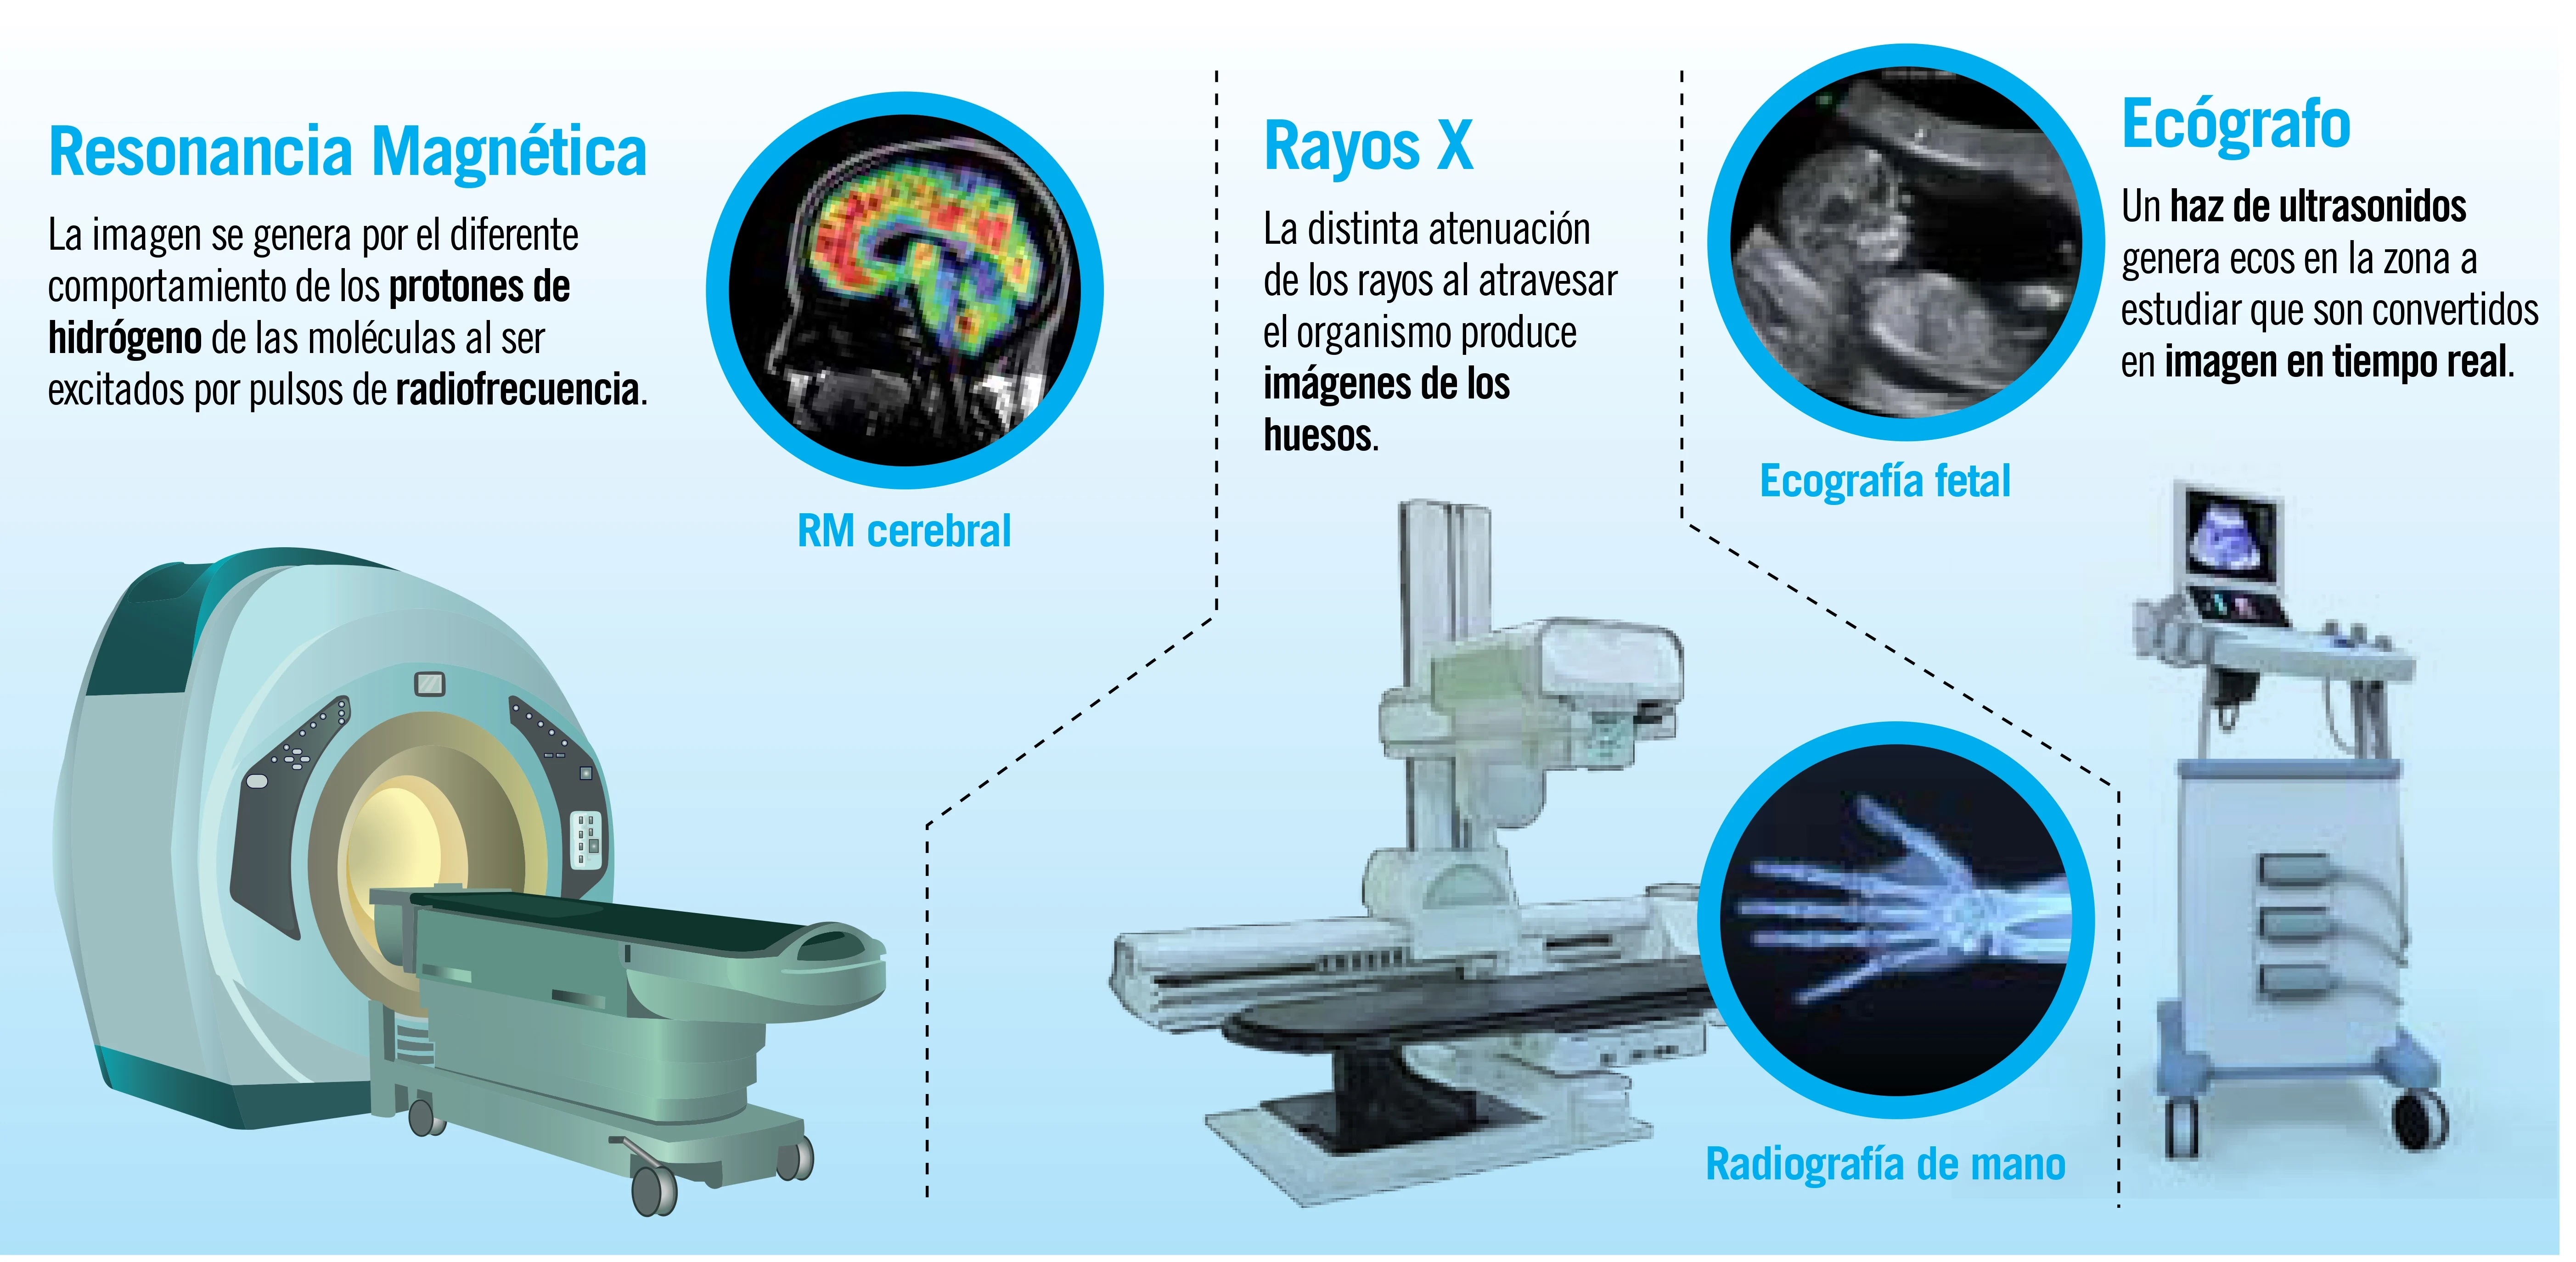
\includegraphics[width=0.7\textwidth]{img/rayosx_vs_rm.png}
    \caption{Comparación esquemática entre rayos X (izquierda) y resonancia magnética (derecha).}
\end{figure}

\subsection{Resonancia Magnética vs. Tomografía Computarizada (TC)}

La tomografía computarizada (TC) también utiliza rayos X, pero en múltiples proyecciones que son reconstruidas mediante algoritmos computacionales, obteniendo imágenes tridimensionales. 
La intensidad detectada en cada ángulo se relaciona con la densidad electrónica del material. 
El proceso de reconstrucción se basa en la \textbf{transformada de Radon} $R[f(x,y)]$:

\begin{equation}
R[f(x,y)](\theta, s) = \int_{-\infty}^{\infty} f(s\cos\theta - t\sin\theta, s\sin\theta + t\cos\theta)\, dt
\end{equation}

y su inversa permite reconstruir la imagen interna del cuerpo.

Por su parte, la RM genera imágenes a partir de la respuesta de relajación de los espines nucleares tras aplicar pulsos de radiofrecuencia. 
Los dos parámetros fundamentales son:

\[
T_1: \text{tiempo de relajación longitudinal}, \quad 
T_2: \text{tiempo de relajación transversal.}
\]

Estos definen el contraste de la imagen según las expresiones:

\begin{align}
M_z(t) &= M_0 \left(1 - e^{-t/T_1}\right), \\
M_{xy}(t) &= M_0 e^{-t/T_2}
\end{align}

donde $M_z$ representa la magnetización en la dirección del campo principal y $M_{xy}$ la componente transversal. 
Mientras la TC resalta diferencias de densidad, la RM distingue variaciones en la composición química y molecular de los tejidos, como el contenido de agua y grasa.

\begin{figure}[h!]
    \centering
    \includegraphics[width=0.7\textwidth]{img/tc_vs_rm.png}
    \caption{Comparación esquemática entre TC y RM.}
\end{figure}

\subsection{Resonancia Magnética vs. Ecografía}

La ecografía utiliza ondas mecánicas (ultrasonido) con frecuencias entre 1 y 15 MHz. 
El principio físico se basa en la reflexión parcial de ondas acústicas en las interfaces de tejidos con distinta impedancia acústica $Z = \rho c$, donde $\rho$ es la densidad y $c$ la velocidad del sonido.

El coeficiente de reflexión se expresa como:

\begin{equation}
R = \left( \frac{Z_2 - Z_1}{Z_2 + Z_1} \right)^2
\end{equation}

Mientras que la RM emplea campos magnéticos y radiofrecuencia, sin involucrar propagación mecánica. 
La ecografía es más adecuada para estudios dinámicos y superficiales (por ejemplo, monitoreo fetal o estructuras musculares), mientras que la RM ofrece mayor resolución en tejidos blandos profundos y análisis espectroscópico.

En términos energéticos, la RM opera en el rango de microondas ($10^7$–$10^8\,\text{Hz}$), con energías asociadas:

\begin{equation}
E = \hbar \omega_0 = \hbar \gamma B_0
\end{equation}

mucho menores que las de los rayos X ($E \approx 10^3$–$10^5\,\text{eV}$), lo que explica su inocuidad radiobiológica.

\section{Conclusiones}

La resonancia magnética se consolida como una de las herramientas más poderosas en el diagnóstico médico contemporáneo. 
Su fundamento físico, basado en la interacción de los momentos magnéticos nucleares con un campo magnético estático $B_0$ y pulsos de radiofrecuencia, permite obtener imágenes de alta resolución sin recurrir a radiación ionizante. 
El principio de Larmor, $\omega_0 = \gamma B_0$, sustenta la selectividad y precisión de esta técnica, lo que la convierte en un método de gran sensibilidad para estudiar tejidos blandos, procesos metabólicos y actividad cerebral.

Los beneficios de la resonancia magnética incluyen su carácter no invasivo, su excelente contraste entre tejidos y la posibilidad de realizar estudios funcionales y espectroscópicos. 
Aplicaciones en neurología, cardiología, oncología y ortopedia demuestran su relevancia clínica y su constante expansión hacia nuevos campos como la resonancia magnética funcional (RMf) y la espectroscopia por RM.

No obstante, el uso de esta tecnología implica ciertas limitaciones y riesgos que deben considerarse. 
El fuerte campo magnético representa un peligro potencial para pacientes portadores de implantes metálicos o marcapasos. 
Asimismo, el uso de contrastes basados en gadolinio puede generar reacciones adversas en individuos con insuficiencia renal, y el alto costo del equipo restringe su acceso en muchos entornos hospitalarios.

En balance, los beneficios superan ampliamente los riesgos cuando la resonancia magnética se emplea de forma responsable y con criterios clínicos adecuados. 
Desde el punto de vista físico, la técnica constituye una aplicación magistral de los principios del magnetismo nuclear y la interacción spin–campo, evidenciando cómo la física moderna puede contribuir directamente al bienestar humano. 
La optimización de tiempos de adquisición, la reducción de ruido y el desarrollo de imanes más eficientes seguirán mejorando la precisión y seguridad de este método, consolidando su papel en la medicina del futuro.

\section{Recomendaciones}

A partir del análisis realizado, se proponen las siguientes recomendaciones orientadas tanto a la práctica clínica como a la investigación y desarrollo de la resonancia magnética:

\subsection{Buenas prácticas para la realización de exámenes de RMN}

Se recomienda que los exámenes de resonancia magnética sean efectuados únicamente por personal capacitado en el manejo de equipos de alto campo magnético. 
Es esencial verificar que el paciente no porte objetos metálicos ni dispositivos electrónicos implantados (como marcapasos o prótesis ferromagnéticas) antes de ingresar a la sala de exploración.  
Asimismo, se debe realizar una adecuada calibración de los gradientes y bobinas de radiofrecuencia para garantizar imágenes precisas y evitar artefactos.

Es conveniente mantener un protocolo de comunicación con el paciente, explicando el procedimiento y el ruido característico del escáner, lo que ayuda a reducir la ansiedad y los movimientos involuntarios durante la adquisición de datos.

\subsection{Precauciones para pacientes y personal médico}

El personal médico debe seguir las normas internacionales de seguridad magnética (IEC 60601-2-33) y las recomendaciones de la \textit{Food and Drug Administration} (FDA).  
En especial, debe controlarse la exposición a campos magnéticos variables y la temperatura corporal del paciente, ya que la radiofrecuencia puede inducir un calentamiento local de los tejidos descrito por la tasa de absorción específica (SAR, \textit{Specific Absorption Rate}):

\begin{equation}
\text{SAR} = \frac{\sigma |E|^2}{\rho}
\end{equation}

donde $\sigma$ es la conductividad eléctrica del tejido, $E$ la amplitud del campo eléctrico inducido y $\rho$ la densidad del material biológico.  
Es recomendable mantener la SAR por debajo de los límites establecidos por la FDA (4\,W/kg en promedio para cuerpo entero).

Además, deben existir zonas de seguridad claramente delimitadas (Zonas I a IV según la normativa ASTM), restringiendo el acceso a personal no autorizado durante la operación del escáner.

\subsection{Recomendaciones para la investigación futura}

Desde la perspectiva científica, se sugiere continuar con el desarrollo de nuevas técnicas de resonancia magnética que optimicen la señal–ruido ($S/N$) y reduzcan los tiempos de adquisición.  
El empleo de imanes de campo ultraalto ($B_0 > 7\,\text{T}$) y algoritmos avanzados de reconstrucción mediante inteligencia artificial ofrecen perspectivas prometedoras para mejorar la resolución espacial y temporal.

Asimismo, la investigación interdisciplinaria entre físicos, ingenieros biomédicos y médicos permitirá explorar nuevas modalidades como la \textit{resonancia magnética cuántica}, la \textit{hiperpolarización de espines nucleares} y la integración con técnicas ópticas o de espectroscopía de terahercios, ampliando el rango de aplicación diagnóstica y terapéutica.

En conclusión, la resonancia magnética seguirá evolucionando como una herramienta esencial de la medicina moderna, en la cual la física desempeña un papel central para garantizar su precisión, seguridad y desarrollo futuro.

\section{Referencias}

\begin{itemize}
    \item Brown, R. W., Cheng, Y.-C. N., Haacke, E. M., Thompson, M. R., \& Venkatesan, R. (2014). 
    \textit{Magnetic Resonance Imaging: Physical and Biological Principles} (4ª ed.). Wiley.

    \item Dawson, M. J. (2013). 
    \textit{Paul Lauterbur and the Invention of MRI}. MIT Press.

    \item Lauterbur, P. C. (1973). 
    Image formation by induced local interactions: Examples employing nuclear magnetic resonance. 
    \textit{Nature, 242}(5394), 190–191.

    \item Mansfield, P. (1977). 
    Multi-planar image formation using NMR spin echoes. 
    \textit{Journal of Physics C: Solid State Physics, 10}(3), L55–L58.

    \item Slichter, C. P. (1990). 
    \textit{Principles of Magnetic Resonance} (3ª ed.). Springer.

    \item Semelka, R. C. (Ed.). (2015). 
    \textit{MRI: Basic Principles and Applications}. Wiley.

    \item Nobel Prize Committee. (2003). 
    The Nobel Prize in Physiology or Medicine 2003: Paul C. Lauterbur and Sir Peter Mansfield. 
    \textit{NobelPrize.org}. Recuperado de \url{https://www.nobelprize.org/prizes/medicine/2003/summary/}

    \item National Center for Biotechnology Information. (2018). 
    Magnetic Resonance Imaging: The Nuclear Option. 
    \textit{PubMed Central}. Recuperado de \url{https://pmc.ncbi.nlm.nih.gov/articles/PMC5988242/}

    \item Huettel, S. A., Song, A. W., \& McCarthy, G. (2015). 
    \textit{Introduction to Functional Magnetic Resonance Imaging: Principles and Techniques} (2ª ed.). Cambridge University Press.

    \item Scott, A. D., et al. (2006). 
    Magnetic Resonance Imaging: Historical Perspective. 
    \textit{Journal of Cardiovascular Magnetic Resonance, 8}(4), 573–580. 
\end{itemize}

\end{document}